\documentclass{article}
\usepackage{amsfonts, amsmath, amssymb, amsthm} % Math notations imported
\usepackage{enumitem}
\usepackage{graphicx}
\usepackage{setspace}
\usepackage{indentfirst}
\usepackage[margin=1in]{geometry}
\graphicspath{{./images/}} % Path to images

% \begin{figure}[htb!]
%      \centering
%      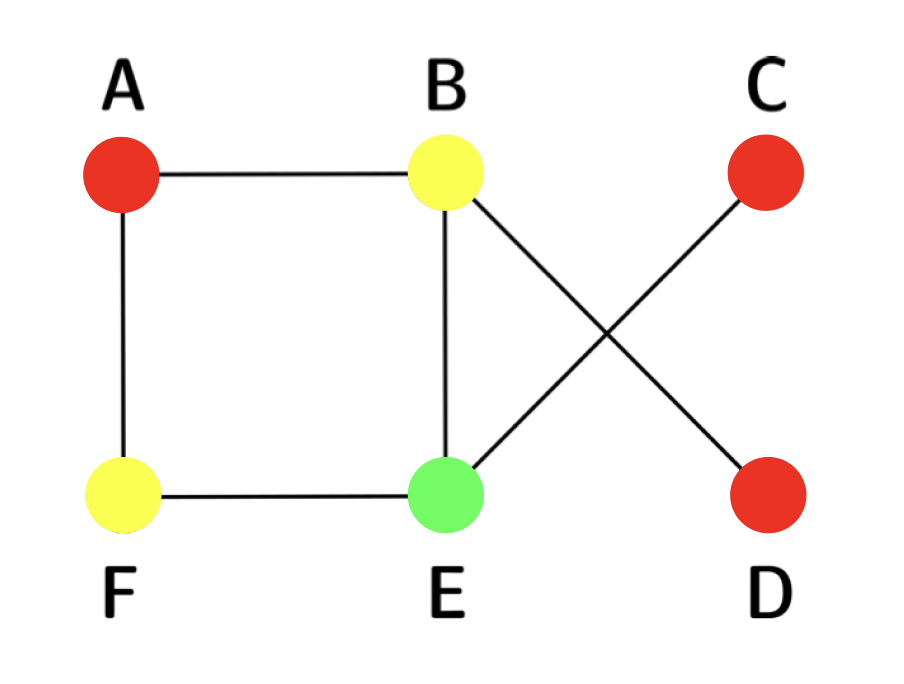
\includegraphics[scale=0.5]{coloring.png}
%      \caption{Coloring of the graph.}
% \end{figure}

% \begin{figure}[htb]
%     \qquad
%     \begin{minipage}{.4\textwidth}
%         \centering
%         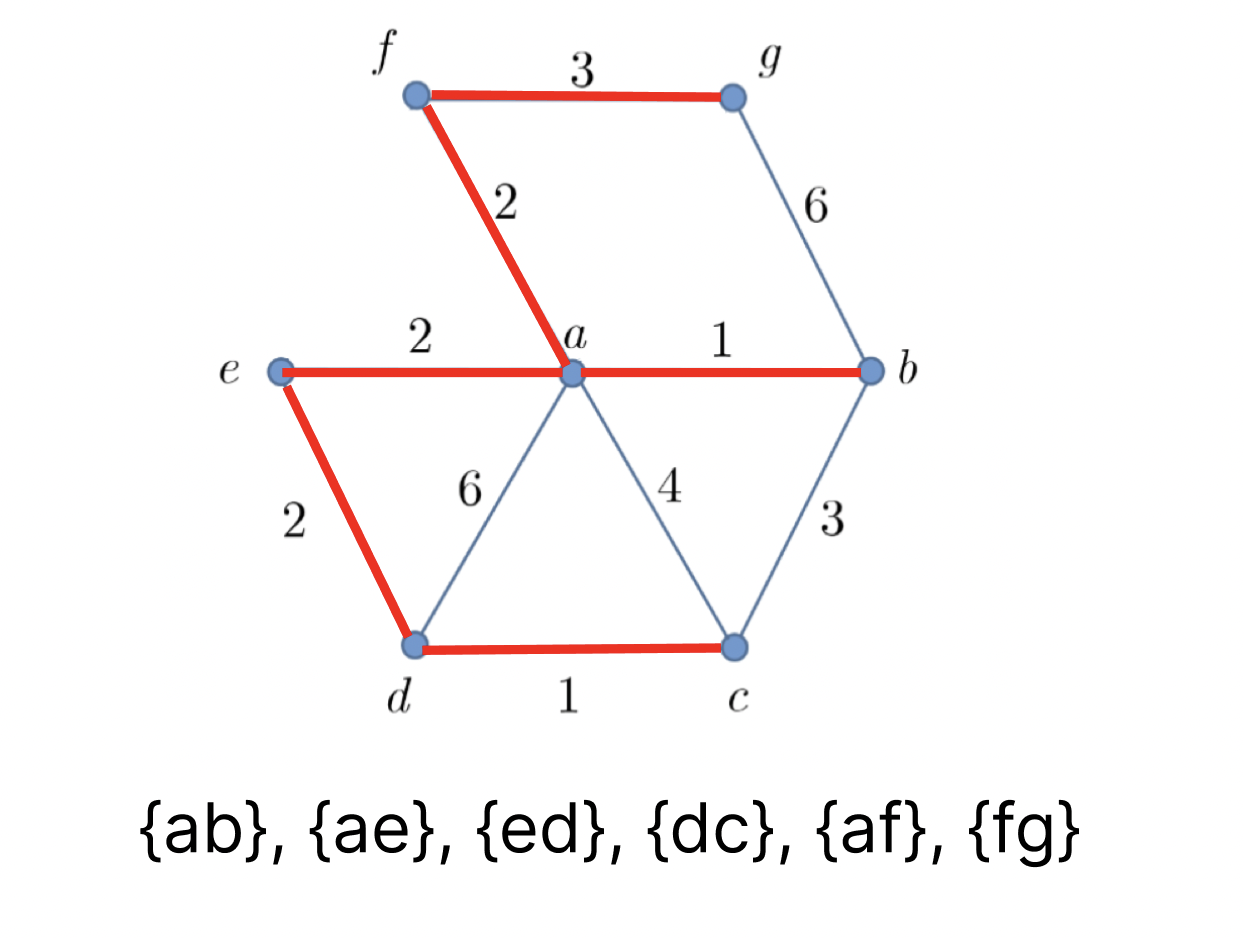
\includegraphics[scale=0.35]{prims.png}
%         \caption{}
%     \end{minipage}    
%     \qquad
%     \begin{minipage}{.4\textwidth}
%         \centering
%         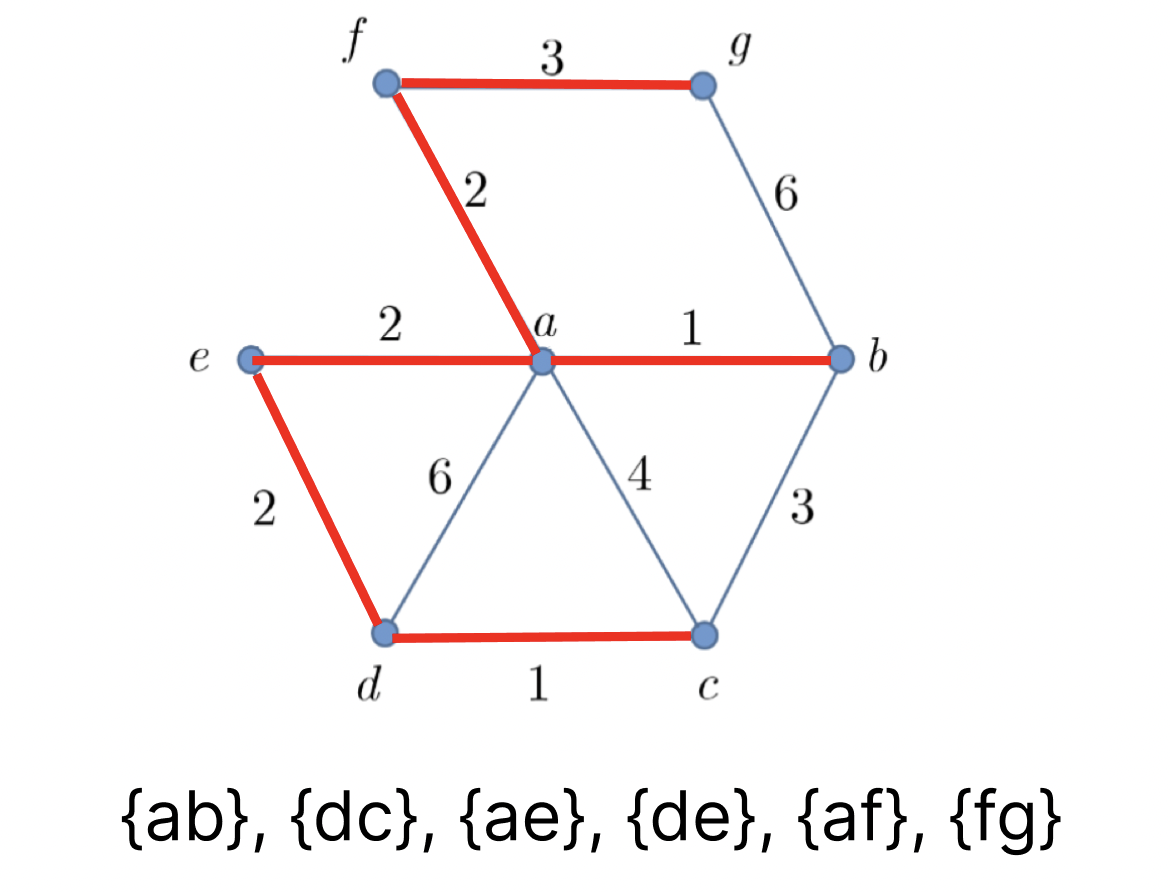
\includegraphics[scale=0.35]{kruskal.png}
%         \caption{}
%     \end{minipage}        
% \end{figure} 

\newtheorem{thm}{Theorem}
\newtheorem{proposition}[thm]{Proposition}
\newtheorem{cor}[thm]{Corollary}

% title information
\title{Math 104 HW4}
\author{Neo Lee}
\date{09/29/2023}

\setstretch{1.15}
% main content
\begin{document} 

% placing title information; comment out if using fancyhdr
\maketitle 

\subsection*{Exercise 9.12}
Assume all $s_n\neq 0$ and that the limit $L=\lim\left|\frac{s_n+1}{s_n}\right|$ exists.
\begin{enumerate}
    \item[\textbf{(a)}]
    \begin{proposition}
        If $L<1$, then $\lim s_n=0$.
    \end{proposition}
    \begin{proof}
        Since $L<1$, $L$ can be written as $L + \delta = 1$ for some $\delta>0$. We know there 
        exists $N$ such that for all $n>N$
        \begin{align*}
            \left|\frac{s_{n+1}}{s_n}-L\right| & < \frac{\delta}{2} \\
            \left|\frac{s_{n+1}}{s_n}\right| & < L + \frac{\delta}{2} = a < 1.
        \end{align*}
        Then, for $n> N$, we have 
        \begin{align*}
            |s_n| & < a^{n-N}|S_N|.
        \end{align*}
        So, now we only have to show that there exists $M$ such that for $n > M, \epsilon>0$, 
        \begin{align*}
            a^{n-N}|S_N| & < \epsilon \\
            a^n & < \frac{\epsilon}{|S_N|}a^N \\
            |a^n| & < \frac{\epsilon}{|S_N|}a^N \\
            |a^n| & < C \qquad (\emph{for some }C>0 ).
        \end{align*}
        Notice $\lim a^n=0$ since $|a|<1$ (Theorem 9.7). So, by definition of limit, indeed there 
        exists such $M$. Therefore, for $n>\max\{M,N\}$, $$|s_n-0| =|s_n| <a^{n-N}|S_N|<\epsilon.$$
    \end{proof}

    \newpage
    \item[\textbf{(b)}]
    \begin{proposition}
        If $L>1$, then $\lim |s_n|=\infty$.
    \end{proposition}
    \begin{proof}
        Define $t_n:=\frac{1}{|s_n|}$. Then, 
        \begin{align*}
            \lim \left|\frac{t_{n+1}}{t_n}\right| & = \lim \left|\frac{s_n}{s_{n+1}}\right| \\
            & = \lim \frac{1}{\left|\frac{s_n+1}{s_n}\right|} \\
            & = \frac{1}{L} < 1.
        \end{align*}
        Hence, from (a), $\lim t_n=0$. Therefore, $\lim |s_n|=\infty$ by Theorem 9.10.
    \end{proof}
\end{enumerate}

\subsection*{Exercise 9.15}
\begin{proposition}
    $\lim_{n\to\infty}\frac{a^n}{n!}=0$ for all $a\in\mathbb{R}$.
\end{proposition}
\begin{proof}
    If $a=0$, then the limit is 0 trivially. If $a\neq 0$, denote $s_n = \frac{a^n}{n!}$, and 
    \begin{align*}
        \left|\frac{s_{n+1}}{s_n}\right| & = \left|\frac{a^{n+1}}{(n+1)!}\frac{n!}{a^n}\right| \\
        \left|\frac{s_{n+1}}{s_n}\right| & = \frac{|a|}{n+1} \\
        \lim_{n\to\infty}\left|\frac{s_{n+1}}{s_n}\right| & = 0.
    \end{align*}
    Then, by (a) of Exercise 9.12, $\lim s_n=0$.
\end{proof}

\subsection*{Exercise 9.18}
\begin{enumerate}
    \item[\textbf{(a)}]
    Verify $1+a+a^2+\cdots+a^n=\frac{1-a^{n+1}}{1-a}$ for $a\neq 1$.
    \begin{proof}[Solution]
        We prove by induction. 

        \emph{Base case:} $n=1$. LHS: $1+a$. RHS: $\frac{1-a^2}{1-a}=\frac{(1-a)(1+a)}{1-a}=1+a$.

        \emph{Inductive step:} Assume the statement is true for $n=k$. Then,
        \begin{align*}
            1+a+a^2+\cdots+a^k+a^{k+1} & = \frac{1-a^{k+1}}{1-a}+a^{k+1} \\
            & = \frac{1-a^{k+1}+a^{k+1}-a^{k+2}}{1-a} \\
            & = \frac{1-a^{k+2}}{1-a}.
        \end{align*}
        Therefore, the statement is true for all $n\in\mathbb{N}$.
    \end{proof}

    \newpage
    \item[\textbf{(b)}]
    Find $\lim_{n\to\infty}(1+a+a^2+\cdots+a^n)$ for $|a|<1$.
    \begin{proof}[Solution]
        \begin{align*}
            \lim_{n\to\infty}(1+a+a^2+\cdots+a^n) & = \lim_{n\to\infty}\frac{1-a^{n+1}}{1-a} \\
            & = \left(\lim 1-a^{n+1}\right) \left(\lim \frac{1}{1-a}\right) \\
            & = \frac{1}{1-a}. \qquad (\because\lim a^{n+1}=0)
        \end{align*}
        Notice, this is just a gerometric series with $r=a$. 
    \end{proof}

    \item[\textbf{(c)}]
    Calculate $\lim_{n\to\infty}\frac{1}{n}\left(1+\frac{1}{3}+\frac{1}{9}+\frac{1}{27}
    +\cdots+\frac{1}{3^n}\right)$.
    \begin{proof}[Solution]
        \begin{align*}
            \lim_{n\to\infty}\frac{1}{n}\left(1+\frac{1}{3}+\frac{1}{9}+\frac{1}{27}
            +\cdots+\frac{1}{3^n}\right) & = \frac{1}{1-1/3} \\
            & = \frac{3}{2}.
        \end{align*}
    \end{proof}

    \item[\textbf{(d)}]
    What is $\lim_{n\to\infty}(1+a+a^2+\cdots+a^n)$ for $a\ge 1$.
    \begin{proof}[Solution]
        For $a\ge 1$,
        \begin{align*}
            \lim_{n\to\infty}(1+a+a^2+\cdots+a^n) \ge \lim_{n\to\infty}(1+1+\cdots+1) 
            & = \lim_{n\to\infty} n+1 \\
            & = \infty.
        \end{align*}
    \end{proof}
\end{enumerate}

\newpage
\subsection*{Exercise 10.6}
\begin{enumerate}
    \item [\textbf{(a)}]
    \begin{proposition}
        Let $(s_n)$ be a sequence such that 
        $$|s_{n+1}-s_n|<2^{-n}\qquad \text{for all } n\in\mathbb{N},$$
        then $(s_n)$ is a Cauchy sequence and hence a convergent sequence.
    \end{proposition}
    \begin{proof}
        We need to show the existence of $N$ such that for all $n,m>N$, $|s_n-s_m|<\epsilon$. 
        Without loss of generality, assume $n\ge m$. Also, $|s_n-s_m|<\epsilon$ is always true 
        for $n=m$ so we consider $n>m$.

        Notice 
        \begin{align*}
            |s_n-s_m| & \le |s_n-s_{n-1}|+|s_{n-1}-s_{n-2}|+\cdots+|s_{m+1}-s_m| \\
            & \le \sum_{k=m}^{n-1}|s_{k+1}-s_k| \\
            & \le \sum_{k=m}^{n-1}2^{-k} \\
            & < \lim_{n\to\infty}\sum_{k=N+1}^{n}2^{-k}.
        \end{align*}
        So now we just need to find $N$ such that $\sum_{k=N+1}^{\infty}2^{-k}<\epsilon$.
        \begin{align*}
            \lim_{n\to\infty}\sum_{k=N+1}^{n}2^{-k} & < \epsilon \\
            \frac{1}{2^{N+1}} + \frac{1}{2^{N+2}} + \cdots & < \epsilon \qquad (\emph{geometric series})\\
            \frac{1}{2^{N+1}} \left(\frac{1}{1-\frac{1}{2}}\right) & < \epsilon \\
            \frac{1}{2^N}  & < \epsilon \\
            2^N & > \frac{1}{\epsilon} \\
            N & > \log_2\frac{1}{\epsilon}.
        \end{align*}
        Hence, we can take $N=\max\{\lceil\log_2\frac{1}{\epsilon}\rceil + 1, 1\}$ and we will get 
        $$|s_n-s_m| < \lim_{n\to\infty}\sum_{k=N+1}^{n}2^{-k} < \epsilon$$
        for all $n,m>N, \epsilon>0$.
    \end{proof}
    
    \item[\textbf{(b)}]
    Is the result in (a) true if we only assume $|s_{n+1}-s_n|<\frac{1}{n}$ for all $n\in\mathbb{N}$.
    \begin{proof}[Solution]
        Not necessarily. Let $s_n=\sum_{k=1}^{n}\frac{1}{2k}$. Then $|s_{n+1}-s_n| = \frac{1}{2n}<
        \frac{1}{n}$ but there does not exists $N$ such that for all $n,m>N$, $|s_n-s_m|<\epsilon$.
        Since $\lim_{n\to\infty}\sum_{N+1}^{n}\frac{1}{2k} = \lim_{n\to\infty}\frac{1}{2}\sum_{N+1}^{n}\frac{1}{k} > 
        \frac{1}{2}\lim_{n\to\infty}\int_{N+1}^{n}\frac{1}{x}dx = \infty$, we can always set 
        $m=N+1$ and find $n$ such that $|s_n-s_m|>\epsilon$.
    \end{proof}
\end{enumerate}

\subsection*{Exercise 10.9}
Let $s_1=1$ and $s_{n+1}=\left(\frac{n}{n+1}\right)s_n^2$ for $n\ge 1$.
\begin{enumerate}
    \item [\textbf{(a)}]
    Find $s_2, s_3, s_4$.
    \begin{proof}[Solution]
        \begin{align*}
            s_2 & = \left(\frac{1}{2}\right)s_1^2 = \frac{1}{2} \\
            s_3 & = \left(\frac{2}{3}\right)s_2^2 = \frac{1}{6} \\
            s_4 & = \left(\frac{3}{4}\right)s_3^2 = \frac{1}{48}.
        \end{align*}
    \end{proof}

    \item[\textbf{(b)}]
    Show $\lim s_n$ exists. 
    \begin{proof}
        Observe that $(s_n)$ is monotonically decreasing, which can be proved by 
        induction. But in fact look at the equation $s_{n+1}=\left(\frac{n}{n+1}\right)s_n^2$ carefuly, 
        $s_n < 1$ starting from $n=2$ so a square of it will only get smaller while $\frac{n}{n+1}$ is 
        always less than 1. So, $s_{n+1}<s_n$ for all $n\ge 2$ [also true for $n=1$].

        Also, $(s_n)$ is bounded below by 0 because every $s_{n+1}$ is defined by multiplication of 
        positive numbers, so $s_{n+1}>0$ for all $n\in\mathbb{N}$.

        Hence, $(s_n)$ is monotonically decreasing and bounded below, so it converges and $\lim s_n$
        exists.
    \end{proof}

    \item[\textbf{(c)}]
    Prove $\lim s_n=0$.
    \begin{proof}
        Notice since $\lim s_n$ exists, we can let $\lim s_n = s = \lim s_{n+1}$. 
        Then according to the recusive definition of $(s_n)$,
        \begin{align*}
            s_{n+1} & = \left(\frac{n}{n+1}\right)s_n^2 \\
            \lim s_{n+1} & = \lim \left(\frac{n}{n+1}\right)s_n^2 \\
            \lim s_{n+1} & = \lim \left(\frac{n}{n+1}\right)\cdot \lim s_n^2 \\
            s & = s^2 \\
            s^2 - s & = 0.
        \end{align*}
        So, $s=0$ or $s=1$. But since $(s_n)$ is monotonically decreasing and $s_2$ is already less 
        than 1, $s=1$ is not possible.

        \emph{Alternatively,} we can prove by using squeeze theorem. We prove by induction that
        $0\le s_n\le\frac{1}{n}$.

        \emph{Base case:} $n=1$. $s_1=1$ and $\frac{1}{1}=1$.

        \emph{Inductive step:} Assume $0\le s_k\le\frac{1}{k}$. Then,
        \begin{align*}
            0 \le s_{k+1} 
            = \left(\frac{k}{k+1}\right)s_k^2 
            \le \left(\frac{k}{k+1}\right)\left(\frac{1}{k}\right)^2 
            = \frac{1}{k(k+1)} \le \frac{1}{k+1}.
        \end{align*}
        Therefore, $0\le s_n\le\frac{1}{n}$ for all $n\in\mathbb{N}$. Then, by squeeze theorem,
        $\lim s_n=0$ because $\lim 0 = 0$ and $\lim \frac{1}{n} = 0$.
    \end{proof}

    \end{enumerate}

\end{document}
